\documentclass[11pt]{standalone}	% Required - Tells LaTeX how to display the document.

\title{Standalone}
\date{May 30th, 2018}
\author{Daniel Borrus}

%% Preamble %%

	\usepackage{inputenc}	% Prepares LaTeX engine for non-ascii characters, such as UTF-8 characters. Important.

	% Page Layout
	%\usepackage{geometry} % set page width
	%\usepackage[margin=1cm]{caption} % set caption width
	%\usepackage{float} % Needed for creating figure “floats”

	% Page Display
	\usepackage{url} % Allows for url links
	\usepackage{graphicx} % Allows for inputing figures
	\usepackage[dvipsnames]{xcolor} % For pretty colors

	% Math Typesetting
	\usepackage{amsmath} % Provides useful equation formats
	\usepackage{amssymb} % Provieds a ton of useful math symbols
	\usepackage{mathtools} % Provides patches for amsmath

	% TikZ/pgfPlots
	\usepackage{tikz}
	\usepackage{pgfplots}
	%\pgfplotsset{compat=1.14}
	\usetikzlibrary{automata,arrows,positioning,calc}
	\pgfplotsset{ every non boxed x axis/.append style={x axis line style=-}, every non boxed y axis/.append style={y axis line style=-}}


\begin{document}

	\centering
	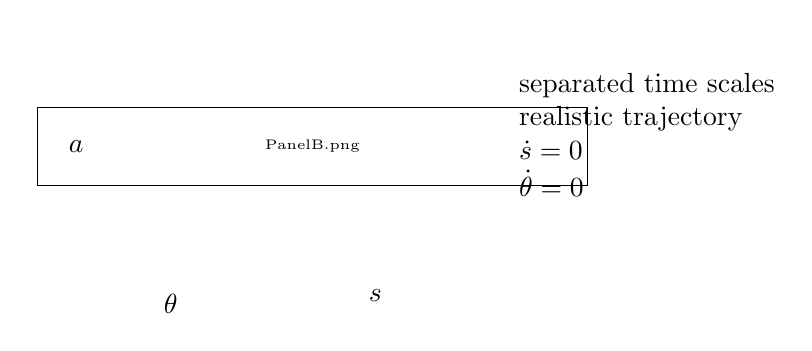
\begin{tikzpicture} 
	
		%\pgfmathsetmacro{\templ}{1998}

		\pgfdeclareimage[width=7cm]{surf}{PanelB.png}
		\node (s) at (0,0) {\pgfuseimage{surf}};
		
		\node at ([shift=({-3cm,0cm})]s) {$a$};
		\node at ([shift=({0.8cm,-1.9cm})]s) {$s$};
		\node at ([shift=({-1.8cm,-2.0cm})]s) {$\theta$};
		
		\draw[fill=white,draw=white] (2,1) -- (2.6,1) -- (2.6,1.5) -- (2,1.5);		
		
		\node[anchor=west] at (2.5,0.77) {separated time scales};
		\node[anchor=west] at (2.5,0.35) {realistic trajectory};	
		\node[anchor=west] at (2.5,-0.05) {$\dot{s}=0$};	
		\node[anchor=west] at (2.5,-0.47) {$\dot{\theta}=0$};				
		
		
	\end{tikzpicture}

\end{document}